\section{Providing Preemption}
\label{sec:preemption}

% \solb{I was thinking of basing the conclusion off this; maybe it should just
% \textit{be} there?}
% 
% \solb{Is it weird to have the following paragraph after we discuss isolation and
% preemption?  I can't think of where else it would go.}
% 
% Our system comprises (1) a central dispatch process that manages the compute node,
% receiving requests and assigning them to (2) a number of worker processes (one per
% dedicated compute core) via a shared memory region.  Each worker process runs a
% tight loop that polls on a ready bit in shared memory; once it finds work to be done,
% it sets itself up to catch any runtime panic and jumps into user code.  The worker
% process receives frequent \texttt{SIGALRM}s to ensure it never loses control of its
% CPU:\ in the associated handler, it checks how for long the current job has been
% running and ends any that has gone over budget.  The rest of this section covers the
% trust model and the preemption scheme.

% <snip>

%\paragraph{Preemption scheme}

The system must be able to detect and recover from microservices that, whether
maliciously or negligently, attempt to run for longer than permitted.  The two parts
of this problem are (1) regaining control of the CPU and (2) aborting and cleaning up
after the user code.

As proposed in Section~\ref{sec:motive}, regaining control of the CPU happens when a
\texttt{SIGALRM} from the kernel transfers control to the worker process's signal
handler.  The handler then checks how long the current microservice has been running
and decides whether it should be killed.  (The handler is registered using the
\texttt{SA\_RESTART} flag to \texttt{sigaction()} so that any interrupted blocking
syscalls are restarted transparently.)

\textbf{For how long should each microservice be allowed to run?}
Let us consider the impact of microservice runtime on tail latency in a well-utilized
but not overloaded compute node, which we'll consider to be one where there is a user
task executing on each available core, but no backlog behind which an incoming task
must wait.
%(This being preliminary work, any discussion of the cluster-level
%scheduling responsible for these theoretical conditions are outside the scope of
%this paper.)
Furthermore, we'll assume an incoming microservice that is warm on each
worker thread.  We define $L$ to be the desired invocation latency, $B$ to be the
compute budget allotted to each microservice, and $r_c$ to be the remaining runtime
of the microservice on CPU $c$.  Thus, in the worst case (where all tasks are
executing for their entire allotted time) the probability that the incoming
microservice will have somewhere to run in time to meet the latency SLO is given by:
\begin{equation}
p(r_\textrm{min} \le L) = \sum\limits_{c \in C} p(r_c \le L) = \big| C \big| \frac{L}{B}
\end{equation}
Given the 14 cores in our setup and imagining we want to keep the 99\% tail
($p(r_\textrm{min} \le L) = 0.99$) to an $L$ of 8 $\mu{}s$, we need to kill tasks
running for more than 113 $\mu{}s$.


\textbf{How often should the handler execute (the \emph{quantum})?}
We showed at the end of Section~\ref{sec:motive} that this is easily
\textit{achievable}, but can it be done \textit{efficiently}?  To find out, we wrote
a microservice that measures the throughput of computing SHA-512 hashes over 64 B of
data at a time.  We then subjected its worker process to \texttt{SIGALRM}s, varying
the quantum and observing the effect on the hashing throughput.
Figure~\ref{fig:hashtput} demonstrates that by a quantum of about 20 $\mu{}s$,
throughput had reached 90\% of baseline.  Considering this an acceptable performance
degradation, we adopt this quantum and prescribe a runtime budget of 93 $\mu{}s$ so
that we can always kill over-budget microservices in time to avoid impacting the tail
latency.

\begin{figure}
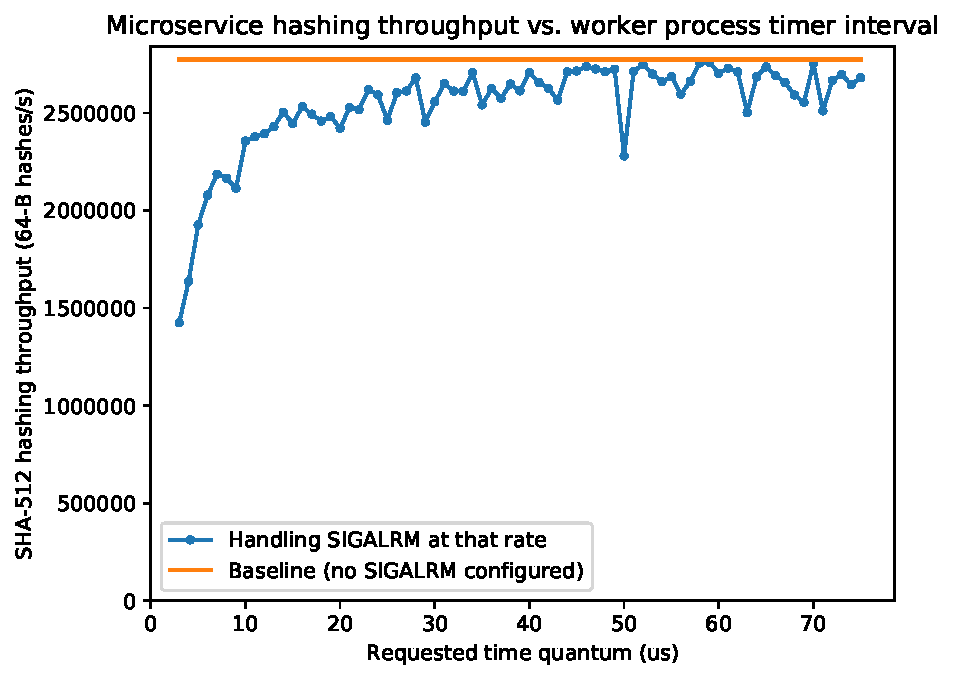
\includegraphics[width=\columnwidth]{figs/2018-02-02-evaluation_quantum-hasher_throughput-throughput}
\caption{Effect of \texttt{SIGALRM} quantum on SHA hashing throughput}
\label{fig:hashtput}
\end{figure}

\textbf{How do we clean up a terminated microservice?}
The problem of regaining control addressed, we now discuss the mechanism for aborting
and cleanup.  POSIX signal handlers receive as one of their arguments a pointer to a
\texttt{ucontext\_t} structure containing a snapshot of the process's PCB (process
control block) the moment before it received the signal.  The most na\"ive way to
regain control would be to reset the GPRs (general-purpose registers) in this
structure to values recorded just before the worker's tight scheduling loop.  The
problem with this approach is that none of the microservice's state or memory
allocations would be expunged from the worker.

One of the few heavyweight components of the Rust runtime is panic handling, which is
reminiscent of C++'s exception handling.  The compiler inserts landing pads into each
function that call the destructors for its variables, and if the program ever panics,
the standard library unwinds the stack, jumping to each landing pad in turn.  We
co-opt this functionality by using the \texttt{SIGALRM} handler to change the context
to describe executing a function that raises an explicit panic in a fake stack frame
just above the real top of the stack.

Note that there are several limitations and security ramifications of our current
approach that would need to be addressed before it was safe to use in a production
environment; for details, see Section~\ref{sec:future}.
